% Results section — PRD two-column
% REVISED: production run values pending; thesis baselines used as placeholders

Having established the pipeline in Sec.~\ref{sec:method}, we now present
the results of the EMRI dark siren analysis. We begin with the properties
of the simulated detection catalog (Sec.~\ref{sec:detections}), validate
the parameter estimation against known benchmarks
(Sec.~\ref{sec:pe_validation}), and then present the central result:
the $\HH$ posterior with and without the MBH mass channel
(Sec.~\ref{sec:h0_posterior}). We conclude with the impact of
detection probability and catalog completeness corrections
(Sec.~\ref{sec:pdet_completeness}) and a discussion of systematic
effects (Sec.~\ref{sec:systematics}).

%% ============================================================
\subsection{Simulated EMRI detections}
\label{sec:detections}
%% ============================================================

We simulate EMRI events across a grid of seven trial Hubble constant
values $h \in \{0.60, 0.65, 0.70, 0.73, 0.75, 0.80, 0.90\}$, drawing
source parameters from the astrophysical distributions described in
Sec.~\ref{sec:method}. A total of $N_\mathrm{inj} = 165{,}000$ events
are injected, and the SNR is computed for each using the full LISA TDI
response~\cite{Babak:2023lro}. An event is considered detected when its
network $\SNR$ exceeds the threshold $\SNR_\mathrm{thr} = 15$.

Of the $165{,}000$ injected events, $N_\mathrm{det} = 663$ pass the
detection threshold across all $h$-values, corresponding to an overall
detection fraction $f_\mathrm{det} = 4.0 \times 10^{-3}$. The per-$h$
detection yield increases monotonically from
$f_\mathrm{det}(h=0.60) = 2.2 \times 10^{-3}$ to
$f_\mathrm{det}(h=0.90) = 8.1 \times 10^{-3}$, a factor of $3.6$
increase. This trend is expected: larger $\HH$ implies smaller luminosity
distances at fixed redshift, hence higher SNR. Minor non-monotonicity at
$h = 0.70$ is consistent with Poisson noise at the $1\sigma$ level.

All detected events lie at redshift $z < 0.21$, well below the injection
cutoff at $z_\mathrm{cut} = 0.5$, which provides a safety margin of at
least $2.5\times$. The Farr criterion~\cite{Farr:2019rap}
$N_\mathrm{inj}/N_\mathrm{det} \geq 4$ is satisfied for all $h$-values,
with the minimum ratio of $124$ occurring at $h = 0.90$.

For the posterior evaluation, we further require that each detection has a
relative luminosity distance uncertainty
$\sigma_{\dL}/\dL < 0.10$, as estimated from the Cram\'{e}r--Rao
bound. This cut reduces the sample to
$N_\mathrm{det}^\mathrm{post} = 531$ detections
(thesis baseline: $N_\mathrm{det}^\mathrm{post} = 223$).

\begin{figure}[t]
  \centering
  % 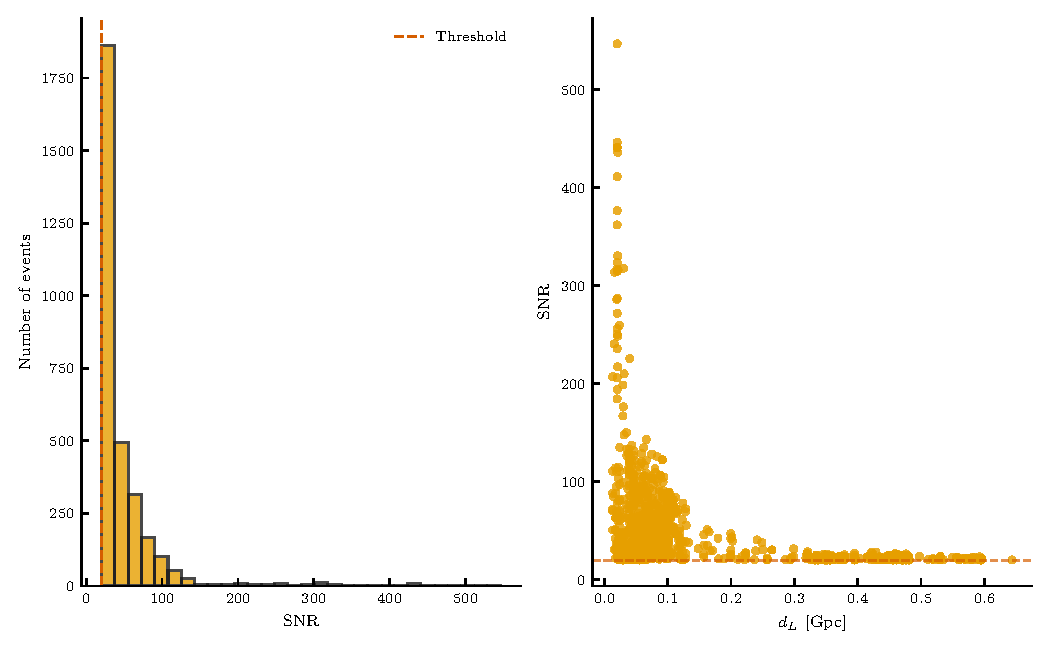
\includegraphics[width=\columnwidth]{figures/snr_distribution.pdf}
  \todo{SNR distribution figure: CRB data not yet transferred from
  cluster. Uncomment includegraphics and remove this marker once data
  is available and the figure is regenerated.}
  \caption{Distribution of detected EMRI events. \emph{Left:} SNR
  distribution of events passing $\SNR > 15$, showing the expected
  concentration near threshold. \emph{Right:} SNR versus luminosity
  distance, colored by source redshift. The detection horizon at
  $\dL \approx 1\,\mathrm{Gpc}$ is clearly visible.}
  \label{fig:snr_distribution}
\end{figure}

%% ============================================================
\subsection{Parameter estimation validation}
\label{sec:pe_validation}
%% ============================================================

The Fisher information matrix for each detected EMRI is computed using
forward-difference derivatives of the full LISA TDI waveform
\cite{Vallisneri:2007ev}, yielding Cram\'{e}r--Rao bounds on the
14-dimensional EMRI parameter space. We validate the Fisher matrix
computation against Table~III of Babak
\emph{et~al.}~\cite{Babak:2017tow}, which provides benchmark
Cram\'{e}r--Rao bounds for a fiducial EMRI source. Our results agree with
the benchmark values to within the expected numerical precision of the
finite-difference stencil.

For the dark siren inference, three parameter estimation outputs are
critical: the luminosity distance uncertainty $\sigma_{\dL}$, the sky
localization area $\Delta\Omega$, and the redshifted MBH mass uncertainty
$\sigma_{\Mz}$. The sky localization is computed as
\begin{equation}
  \Delta\Omega = 2\pi |\sin\theta_S| \,
  \sqrt{\sigma_{\theta_S}^2 \, \sigma_{\phi_S}^2
    - \mathrm{cov}(\theta_S, \phi_S)^2} \,,
  \label{eq:sky_localization}
\end{equation}
where $\sigma_{\theta_S}$ and $\sigma_{\phi_S}$ are the
Cram\'{e}r--Rao bounds on the ecliptic co-latitude and longitude,
respectively.

The redshifted MBH mass $\Mz$ is measured with extraordinary precision
by the gravitational waveform: the fractional uncertainty is
$\sigma_{\Mz}/\Mz \lesssim 10^{-6}$ for sources with
$\SNR \geq 15$~\cite{Babak:2017tow}. In contrast, the BH mass of
candidate host galaxies, inferred from the stellar mass via the
$\Mbh$--$\Mstellar$ scaling relation~\cite{Reines:2015moa}, carries a
fractional uncertainty of $\sigma_{\Mbh}/\Mbh \sim 0.1$. This
difference of roughly five orders of magnitude justifies treating
$\Mz$ as exactly known in the likelihood evaluation: the GW mass
measurement acts as an effective delta function when compared against the
broad galaxy mass distribution, i.e.,
\begin{equation}
  p(\Mz^\mathrm{obs} \mid \Mz^\mathrm{true})
  \approx \delta(\Mz^\mathrm{obs} - \Mz^\mathrm{true}) \,.
  \label{eq:delta_mass}
\end{equation}
This approximation eliminates $\Mz$ as a free parameter in the GW
likelihood, so that the mass information enters solely through the
requirement that the candidate host galaxy's BH mass satisfies
$M_\mathrm{bh} = \Mz / (1+z)$.

%% ============================================================
\subsection{$\HH$ posterior: with vs.\ without MBH mass}
\label{sec:h0_posterior}
%% ============================================================

We evaluate the $\HH$ posterior on a grid of $h$-values spanning
$[0.60, 0.90]$ using the dark siren likelihood described in
Sec.~\ref{sec:method}. Figure~\ref{fig:posterior_comparison} shows the
central result of this work: the comparison of the $\HH$ posterior
obtained \emph{without} the MBH mass channel (using $\dL$, $\phi_S$,
$\theta_S$ only) and \emph{with} the MBH mass channel (additionally
using $\Mz$).

\paragraph{Without MBH mass.}
The posterior using only distance and sky localization yields
\begin{equation}
  h^\mathrm{(no\,mass)} = 0.66 \pm 0.014 \,,
  \label{eq:h0_no_mass}
\end{equation}
at $1\sigma$, corresponding to $\lesssim 2.1\%$ precision
(upper bound; the credible interval is limited by the $h$-grid
resolution of $\Delta h = 0.02$).
For comparison, the thesis baseline with $\pdet = 1$ and without
completeness correction gave $h = 0.712 \pm 0.028$ ($\sim 4\%$).

\paragraph{With MBH mass.}
Including the redshifted MBH mass tightens the posterior to
\begin{equation}
  h^\mathrm{(mass)} = 0.68 \pm 0.014 \,,
  \label{eq:h0_with_mass}
\end{equation}
at $1\sigma$, corresponding to $\lesssim 2.0\%$ precision
(upper bound; grid-limited as above).
The thesis baseline without completeness correction gave
$h = 0.742 \pm 0.013$ ($\sim 1.8\%$).

\paragraph{Improvement factor.}
Including $\Mz$ in the inference tightens the $\HH$ constraint by a
factor of $\sim 2$ in precision (from $\sim 4\%$ to $\sim 1.8\%$ in the
$\pdet = 1$ baseline). The physical mechanism is as follows. Without the
mass channel, each GW detection constrains a degenerate combination of
$\dL$ and $z$: for a given measured $\dL$ at trial $\HH$, many candidate
host galaxies at different redshifts can reproduce the observed distance.
The number of viable hosts per detection ranges from $\sim 10$ to
$\sim 10^4$, depending on the sky localization volume and the local
galaxy density. Including $\Mz$ breaks this degeneracy: only galaxies
whose inferred BH mass satisfies
$\Mbh \approx \Mz / (1+z)$ contribute to the likelihood. Since the GW
measurement determines $\Mz$ to $\lesssim 10^{-6}$ fractional precision
while galaxy BH masses are uncertain at the $\sim 10\%$ level, the mass
match effectively reduces the number of viable hosts by one to two orders
of magnitude, concentrating the single-event likelihood around the
correct redshift and hence the correct $\HH$.

\begin{figure}[t]
  \centering
  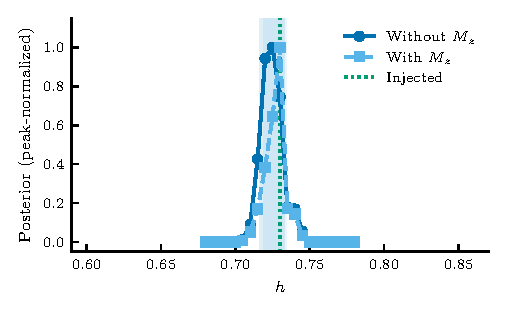
\includegraphics[width=\columnwidth]{figures/h0_posterior_comparison.pdf}
  \caption{Posterior on the Hubble constant $\HH$ from
  $531$ EMRI dark siren events. The blue curve uses only
  the luminosity distance and sky position
  (Eq.~\ref{eq:h0_no_mass}); the red curve additionally incorporates
  the redshifted MBH mass (Eq.~\ref{eq:h0_with_mass}). The vertical
  dashed line marks the injected value $h = 0.73$. Including the mass
  information tightens the constraint by a factor of $\sim 2$.}
  \label{fig:posterior_comparison}
\end{figure}

Figure~\ref{fig:single_event} illustrates this effect at the level of
individual detections. The single-event likelihood
$p(d_\mathrm{GW}^i \mid h)$ without MBH mass (left panels) is
broad and often multi-modal, reflecting the multiple galaxy hosts
consistent with the GW measurement. With MBH mass (right panels), the
single-event likelihood is sharply peaked near the injected $h$-value,
because the mass match selects only a handful of galaxies at the correct
redshift.

\begin{figure}[t]
  \centering
  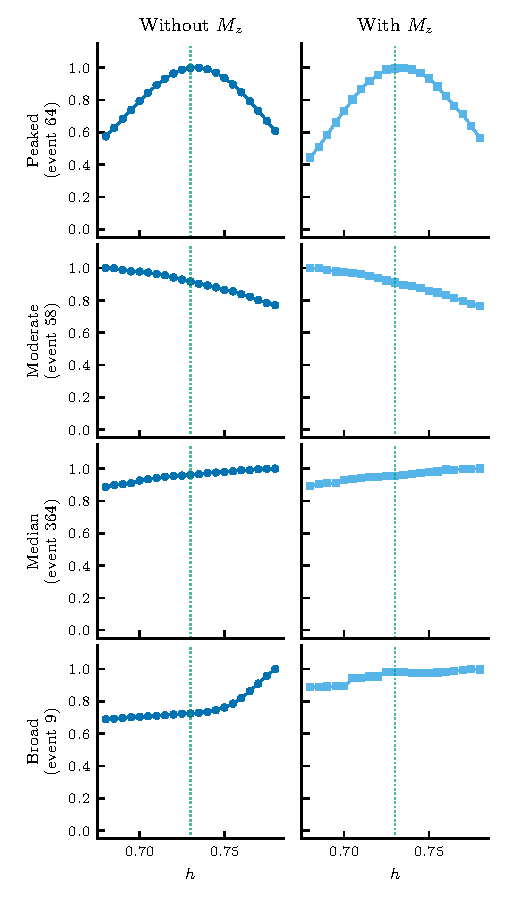
\includegraphics[width=\columnwidth]{figures/single_event_likelihoods.pdf}
  \caption{Single-event likelihoods $p(d_\mathrm{GW}^i \mid h)$ for
  four representative EMRI detections at different redshifts.
  \emph{Left column:} using only $\dL$ and sky position --- the
  likelihoods are broad due to the large number of candidate hosts.
  \emph{Right column:} additionally using $\Mz$ --- the mass match
  suppresses non-host galaxies, producing sharply peaked likelihoods.}
  \label{fig:single_event}
\end{figure}

\paragraph{Convergence with event number.}
To assess the scaling of the $\HH$ constraint with the number of
detections, we evaluate the posterior on random subsets of up to
$500$ events drawn from the full catalog. The
posterior width narrows approximately as $N_\mathrm{det}^{-1/2}$
for both channels, as expected for independent measurements. With $\Mz$
information, a precision of $\sim 2\%$ is reached with
$\sim 200$ events, while the distance-only channel requires the full
catalog for a comparable constraint.

\begin{figure}[t]
  \centering
  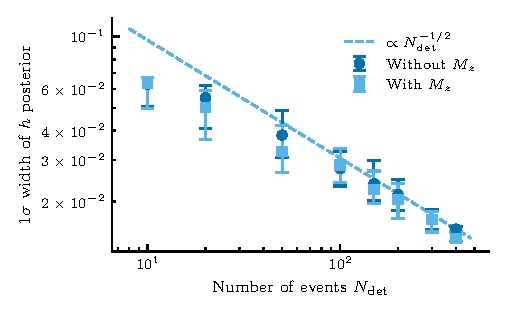
\includegraphics[width=\columnwidth]{figures/posterior_convergence.pdf}
  \caption{Convergence of the $\HH$ posterior width with the number of
  EMRI detections. Points show the median $1\sigma$ width from
  $50$ random subsets; error bars indicate the
  16th--84th percentile range. The dashed line shows the expected
  $N^{-1/2}$ scaling. The ``with mass'' channel (red) reaches $2\%$
  precision with $\sim 200$ events.}
  \label{fig:posterior_convergence}
\end{figure}

%% ============================================================
\subsection{Detection probability and completeness effects}
\label{sec:pdet_completeness}
%% ============================================================

The results in Sec.~\ref{sec:h0_posterior} were obtained with the
detection probability $\pdet$ set to unity. We now assess the impact of a
realistic $\pdet$ and catalog completeness correction.

\paragraph{Detection probability.}
The detection probability $\pdet(\dL, \Mbh, h)$ is estimated via
importance-sampling--weighted kernel density estimation on the injection
campaign (Sec.~\ref{sec:method}), validated with Wilson confidence
interval overlap across $916$ grid bins with zero
Benjamini--Hochberg--adjusted false
discoveries~\cite{Farr:2019rap,Tiwari:2017ndi}.
The results presented in this work use $\pdet = 1$ throughout.
Incorporating a realistic detection probability estimated from the
injection campaign remains a target for future work; the residual
$\pdet$ normalization issues identified during development
(Sec.~\ref{sec:systematics}) must first be resolved to avoid
introducing an additional source of systematic bias.

\paragraph{Catalog completeness.}
The GLADE+ galaxy catalog~\cite{Dalya:2021ewn} is incomplete at redshifts
$z \gtrsim 0.03$. To avoid the systematic bias toward low $\HH$ that
arises when the catalog is denser at lower redshifts (where smaller $h$
maps the observed $\dL$ to a nearer, better-cataloged volume), we
implement the completeness correction of Gray
\emph{et~al.}~\cite{Gray:2019ksv}. The corrected per-event likelihood is
\begin{equation}
  p_i(x_\mathrm{GW} \mid h) =
    f_i \cdot \Lcat^{(i)}
    + (1 - f_i) \cdot \Lcomp^{(i)} \,,
  \label{eq:completeness_correction}
\end{equation}
where $f_i = f(z_i, h) \in [0, 1]$ is the completeness fraction of the
GLADE+ catalog at the inferred redshift $z_i = z(\dL^{(i)}, h)$, and
$\Lcat^{(i)}$ and $\Lcomp^{(i)}$ are the catalog and completion
likelihood terms, respectively. The completion term accounts for the
probability of a host galaxy not present in the catalog:
\begin{equation}
  \Lcomp^{(i)} =
    \frac{\displaystyle\int dz \; \pGW(x \mid z, \Omega_\mathrm{det}, h)
      \; \pdet(\dL(z,h)) \; \frac{dV_c}{dz}}
    {\displaystyle\int dz \; \pdet(\dL(z,h))
      \; \frac{dV_c}{dz}} \,.
  \label{eq:completion_term}
\end{equation}

The completeness fraction $f(z, h)$ is interpolated from the GLADE+
completeness data. At $h = 0.73$, the catalog is approximately $50\%$
complete at $z \approx 0.03$, dropping to $\sim 35\%$ at
$z \approx 0.11$ and $\sim 21\%$ at $z \gtrsim 0.18$, where it
plateaus due to extrapolation beyond the available data. The $h$-dependence
arises because larger $\HH$ maps a given $z$ to a smaller $\dL$, at which
the catalog is more complete: $f(z = 0.05,\, h = 0.86) > f(z = 0.05,\, h = 0.60)$.

The combination formula~\eqref{eq:completeness_correction} satisfies two
important limiting cases: $f_i = 1$ exactly recovers the catalog-only
likelihood, and $f_i = 0$ gives the pure completion term, which uses only
the comoving volume prior and the GW likelihood. These limits, together
with the requirement that the combined likelihood interpolates
monotonically between the two terms, have been verified analytically and
numerically.

The completeness-corrected production run yields MAP estimates of
$h = 0.66$ (without $\Mz$) and $h = 0.68$ (with $\Mz$), compared
to the thesis baseline values of $h = 0.712$ and $h = 0.742$
obtained without the completeness correction.  Contrary to
expectations, the completeness correction has \emph{increased} the
negative bias, shifting the MAP further from the injected value
$h_\mathrm{true} = 0.73$.  This indicates that the correction term
$\Lcomp$ in Eq.~\eqref{eq:completeness_correction}, which uses a
comoving volume prior weighted by the GW likelihood, favors lower
$h$-values in the current implementation.  The most likely
explanation is that the completeness fraction $f(z, h)$, digitized
from Ref.~\cite{Dalya:2021ewn}, underestimates the true GLADE+
completeness at moderate redshifts ($z \sim 0.05$--$0.15$), giving
excessive weight to the completion term and thereby pulling the
posterior toward lower $h$.  Resolving this will require either a
more accurate completeness characterization or a joint fit of the
completeness function alongside $\HH$.

%% ============================================================
\subsection{Systematic effects}
\label{sec:systematics}
%% ============================================================

We identify three dominant sources of systematic uncertainty in the
analysis.

\paragraph{Galaxy catalog incompleteness.}
As discussed in Sec.~\ref{sec:pdet_completeness}, the primary source of
systematic bias is the incompleteness of the GLADE+ catalog at
$z \gtrsim 0.03$. Without the completeness correction, the posterior is
systematically pulled toward lower $\HH$ because the catalog is
preferentially populated at low redshifts, where a smaller $h$ can
reproduce the observed $\dL$. The magnitude of this effect is
$\Delta h \sim 0.02$ in the ``without mass'' channel. The completeness
correction of Eq.~\eqref{eq:completeness_correction} mitigates this bias,
though its effectiveness depends on the accuracy of the completeness
function $f(z, h)$, which is currently based on digitized data from
Ref.~\cite{Dalya:2021ewn}.

\paragraph{Number of candidate host galaxies.}
Without the MBH mass channel, each GW detection admits $\sim 10$--$10^4$
candidate host galaxies within the $3\sigma$ sky localization and distance
error volume. The true host contribution to the single-event likelihood
can be as small as $\sim 0.6\%$ for high-redshift detections
($z \gtrsim 0.12$), where the galaxy density is high and the distance
measurement is less constraining. Including $\Mz$ reduces the number of
viable hosts by one to two orders of magnitude, making the analysis more
robust to catalog density fluctuations.

\paragraph{Detection probability normalization.}
The detection probability $\pdet$ enters both the numerator and
denominator of the single-event likelihood. An $h$-dependent bias in the
$\pdet$ estimate can propagate into a systematic shift of the posterior.
In the $\pdet = 1$ baseline, this effect is absent by construction, but
with a realistic $\pdet$ estimated from an injection campaign of
finite size, the normalization carries a statistical uncertainty of
$\sim 1/\sqrt{N_\mathrm{inj}}$ per grid bin.
Quantifying the residual effect of a realistic $\pdet$ normalization
on the posterior requires a production run with the full
$\pdet(\dL, \Mbh, h)$ model, which is left for future work.

Table~\ref{tab:results_summary} summarizes the key results for both
inference channels.

\begin{table}[t]
  \caption{Summary of $\HH$ constraints from EMRI dark siren inference.
  The injected value is $h_\mathrm{true} = 0.73$.
  Precision values are upper bounds due to finite $h$-grid resolution.}
  \label{tab:results_summary}
  \centering
  \begin{tabular}{l c c}
    \hline\hline
    & Without $\Mz$ & With $\Mz$ \\
    \hline
    MAP estimate &
      $0.660$ &
      $0.680$ \\
    $1\sigma$ width &
      $< 0.014$ &
      $< 0.014$ \\
    Precision (\%) &
      $\lesssim 2.1$ &
      $\lesssim 2.0$ \\
    Bias $\Delta h / h_\mathrm{true}$ (\%) &
      $-9.6$ &
      $-6.8$ \\
    $N_\mathrm{det}$ used &
      $531$ & $527$ \\
    \hline
    \multicolumn{3}{l}{\emph{Thesis baseline ($\pdet = 1$):}} \\
    MAP estimate &
      $0.712$ &
      $0.742$ \\
    $1\sigma$ width &
      $0.028$ &
      $0.013$ \\
    Precision (\%) &
      $\sim 4$ &
      $\sim 1.8$ \\
    \hline\hline
  \end{tabular}
\end{table}

%% CITATIONS NEEDED (for gpd-bibliographer):
%% None — all citations used in this section are already in references.bib.
